%!TEX root = ../report.tex
\documentclass[report.tex]{subfiles}
\begin{document}
    \chapter{Comprehensive study of Selected algorithms}

    From the 3D semantic SLAM methods, we are selecting QuadricSLAM and OA-SLAM methods to look into the backend pipeline, understand the implementation details and identify the challenging sections within it. Also, the evaluation of such object-oriented SLAM methods are also performed.


    \section{QuadricSLAM}
    \subsection{Summary}
\begin{figure}[H]
\centering
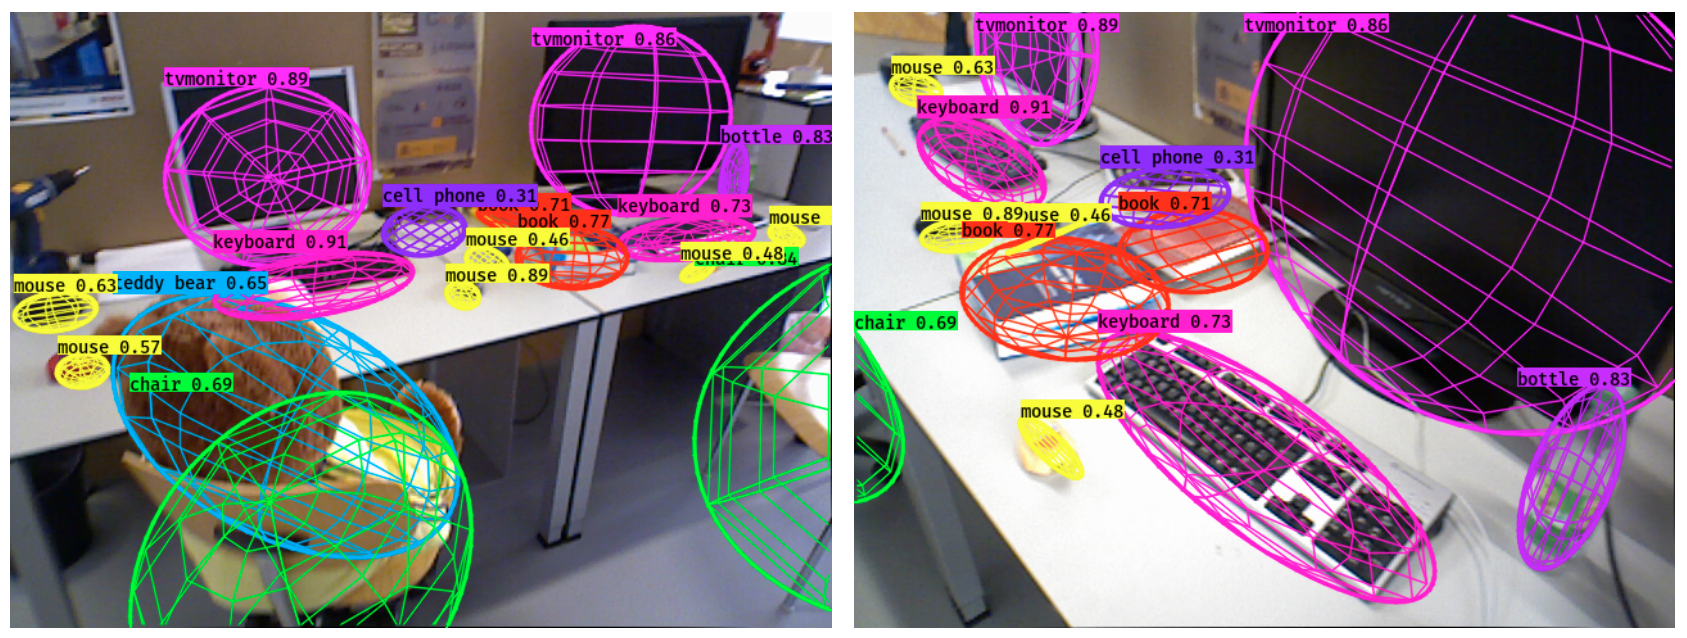
\includegraphics[width=\textwidth, height=0.3\textheight] {Images/Quadric_slam.png}
\caption{\centering\textbf{QuadricSLAM}: Ellipsoids fitted on objects in image plane\cite{quadric2}}
\label{fig:QuadricSLAM}
\end{figure}
    
\begin{itemize}
\item The Quadric SLAM is a semantic SLAM approach where each object within the environment is represented using dual quadrics whose parameters are estimated and optimised using multi-view geometry.
\item The optimisation is based on the 2D bounding box generated for each object observed at different view points. This object detection method also helps to add semantic label to each object.
\item SLAM involves performing mapping and robot pose estimation in a combined fashion. Here the robot camera poses and the quadric parameters are estimated using underlying factor graph based back-end. The odometry errors in the factor graph could be reduced through the loop closure which is aided by re-observing the quadric representation of the object at different view points. Thus both the odometry and the observation are aiding to minimize the errors of each other.
\item In the initial paper released by the authors \cite{sünderhauf2017dual}, a monocular perspective camera was used to input RGB images to the front-end of the framework without any depth information.
\item The quadric used in this application is ellipsoid because its a closed surface. It can capture the position(3 parameters), radius or size(3 parameters) and orientation(3 parameters) of the object in the 3D world. This kind of representation can help to reduce the memory required to store the dense 3D representation of the surface of the object and at the same time serves all the basic purposes like object pose estimation, localization, semantic navigation and planning tasks.
\item The following section explains about the mathematics behind dual quadric representation. The section is a summarized version of the content in section 3 of the Quadric SLAM paper\cite{sünderhauf2017dual}.
\item For each view of an object, a 2D bounding box is generated with 4 corners $x_{1}, x_{2}, x_{3}$ and $x_{4}$. Each one can be represented using a 3D homogeneous vector.
\item Further, the 4 edges of the bounding box $l_{1}, l_{2}, l_{3}$ and $l_{4}$ can be represented as a cross product of these corner points. $l_{1} = x_{1} X x_{2}, l_{2} = x_{2} X x_{3}, l_{3} = x_{3} X x_{4}$ and $l_{4} = x_{4} X x_{1}$.
\item The lines drawn from the camera center to each of the four corner points can back-project the four edge lines into four 3D planes. The equation of the 3D plane can be written as $\pi_{i} = P^{T}l_{i}$ where i is the index of the 2D edge for which the 3D plane is generated. P is the camera projection matrix, P = K[R t] where K is the intrinsic parameter matrix of size 3x3 and R and t are the extrinsic parameter matrix of the camera of size 3x4. Therefore P is a matrix of size 3x4 and the resultant 3D plane $\pi_{i}$ is a 4D homogeneous vector.
\item Thus a single view can create a constrained 3D space enveloped by four 3D planes. Since we don't have an enclosed 3D region from a single view, we may need multiple views to further constrain the object's shape and orientation.

\begin{figure}[H]
\centering
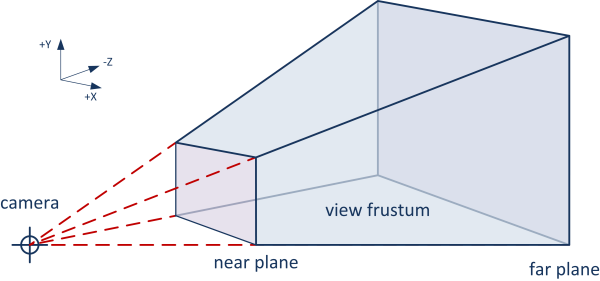
\includegraphics[width=\textwidth, height=0.3\textheight] {Images/VisualCameraFrustum.png}
\caption{\centering Back projection of 2D bounding box \href{https://learnopengl.com/img/guest/2021/Frustum_culling/VisualCameraFrustum.png}{[ref]}}
\label{fig:frustum}
\end{figure}

\item In the above figure \ref{fig:frustum}, we can see the bounding box which is represented as the near plane which is back-projected to infinity. The view frustum area is the most probable area where the object can be located. To form a closed region from these 3D view frustums, we need at least 3 views which can be seen in the figure \ref{fig:enclosure} below.

\begin{figure}[H]
\centering
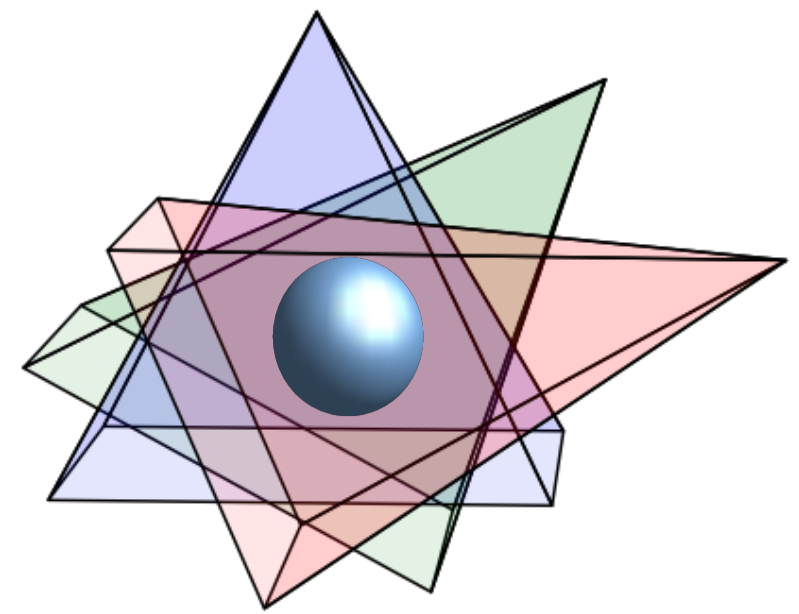
\includegraphics[width=0.35\textwidth, height=0.3\textheight] {Images/enclosure.png}
\caption{\centering Closed region by 3 view frustums}
\label{fig:enclosure}
\end{figure}

\item The next important concept is what and how to represent a quadric. A quadric Q is a 3D surface that is characterized by a set of points $x$ on the surface that satisfies the equation $x^{T}Qx = 0$. Q is a 4x4 symmetric matrix.
\item The same equation can be rewritten in terms of tangential planes that passes through each of these points that can create an closing envelope around the surface. $\pi^{T}Q^{*}\pi = 0$. $Q^{*}$ is called as dual quadrics or dual representation of the quadric which is calculated by $Q^{*} = Q^{-1}$ if Q has an inverse or $Q^{*} = adjoint(Q)$.
\item Since $Q^{*}$ is a symmetric 4x4 matrix, there are 10 unique elements. Three for centroid, three for size or radius, three for orientation and one for scaling factor which is usually kept constant as -1. So only need to optimize for 9 parameters. $Q^{*}$ can be represented as $Q^{*} = T Q^{*}_{0} T^{T}$ where $Q^{*}_{0}$ is the representation of an ellipsoid centered at origin and T is the homogeneous transformation matrix of size 4x4 involving a rotation and translation parameter [R t] to transform the ellipsoid from origin.
$$
 Q^{*}_{0}
 =
  \begin{bmatrix}
   r_1^2 & 0 & 0 & 0 \\
   0 & r_2^2 & 0 & 0 \\
   0 & 0 & r_3^2 & 0 \\
   0 & 0 & 0 & -1
   \end{bmatrix}
$$
\item The parameters $r_1, r_2$ and $r_3$ governs the size or radius of the ellipsoid. The orientation and centroid parameters are incorporated as rotation and translation parameters in the homogeneous transformation matrix T. After matrix multiplication, the matrix $Q^{*}$ turns into a transformation matrix where the centroid is the last column of $Q^{*}$ as a homogeneous 4x1 vector. The orientation parameters pitch, yaw, roll has to be extracted from the first 3x3 dimension of the dual quadric matrix.
\item The above concept of $\pi_{i}^{T}Q^{*}\pi_{i} = 0$ represents an 3D equation. However the bounding box observations we obtained from the detectors are in 2D. We have to convert from quadrics to conics which is ellipsoids to ellipses in this case. The dual conics $C^{*}$ can be written as $C^{*} = P Q^{*} P^{T}$ where the 3D ellipsoid $Q^{*}$ is projected onto the 2D image plane using the camera projection matrix P mentioned before.
\item The definition of quadrics also remains same for conics $x^{T}Cx = 0$ where x is now replaced with 2D points. And as tangential planes exists for points in 3D, tangential lines exists for points in 2D. Hence $\pi^{T}Q^{*}\pi = 0$ for quadrics could be replaced by $l^{T} C^{*} l = 0$ for conics where $C^{*}$ is the dual conic representation and $l$ is the set of tangential lines.
\item Substituting the expression for dual conics in the above equation yields, $l^{T} P Q^{*} P^{T} l = 0$.
\item Per detection of an object from a view point, the bounding box generates 4 lines which can act as 4 constraints on the dual quadrics. For dual quadrics $Q^{*}$, there are 9 unknown parameters and atleast 3 observations from different view points are needed to generate a solution for the same.
\begin{figure}[H]
    \centering
    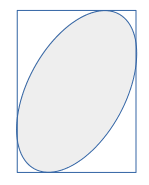
\includegraphics{Images/bbox.png}
    \caption{Four tangential lines to the object conic ellipse}
    \label{fig:bbox}
\end{figure}

\item Internally, the quadricSLAM has the virtual representation of the 3D environment and when the camera pose comes back to already mapped object, the 2d view of the 3D object is projected onto the image plane as in figure \ref{fig:QuadricSLAM}. The concept is similar to the image \ref{fig:3d2dprojection} below except that in our case, the 3D object is ellipsoid and the 2D projection is ellipse.

\begin{figure}[H]
\centering
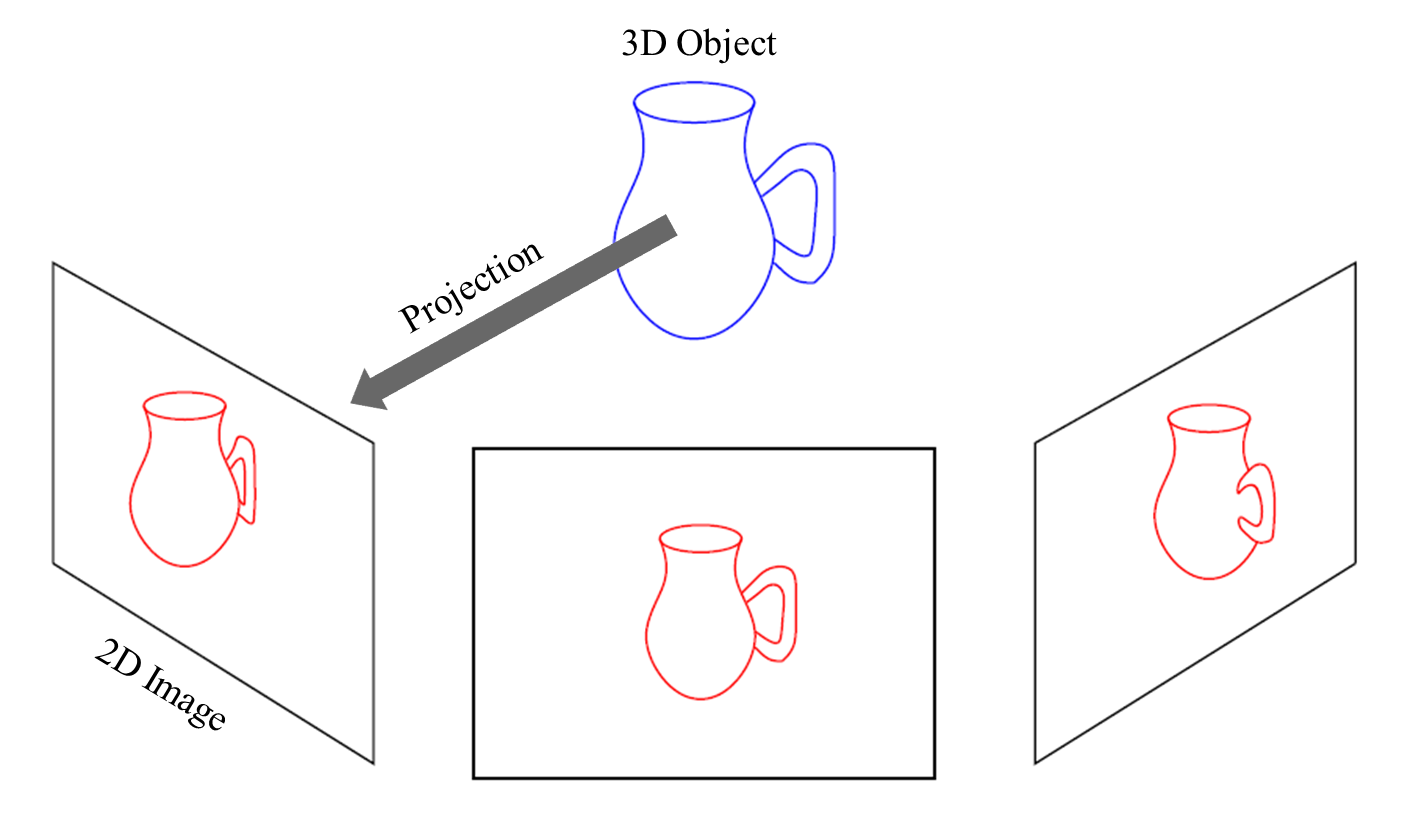
\includegraphics[width=\textwidth, height=0.3\textheight] {Images/3d_2d_view.png}
\caption{\centering 3D virtual scene to 2D image plane projection \href{http://2.bp.blogspot.com/-jhez8PBjdXo/UO0wQk9xl9I/AAAAAAAAASE/3eXxHntYxT4/s1600/fig1.png}{[ref]}}
\label{fig:3d2dprojection}
\end{figure}

\item The following section explains about the mathematics behind using the dual quadric representation in SLAM backend for optimization and corrections. The section is a summarized version of the content in section 4 of the Quadric SLAM paper\cite{sünderhauf2017dual}.

\item To define the factor graph, we define certain parameters for the odometry and observations:
\begin{itemize}
    \item A set of robot camera poses X = \{$x_i$\} where i is the index of the pose at which a particular observation is made.
    \item A set of landmarks Q = \{$q_j$\} where $q_j$ indicates the dual quadric representation for the object j.
    \item A set of observations U = \{$u_i$\} where $u_i$ is the odometry data available via wheel odometry or visual odometry.
    \item A set of lines L = \{$l_ijk$\} where k ranges from 0 to 4. $l_ijk$ denotes the line k of the bounding box for object j being viewed at pose i.
\end{itemize}

\item The conditional probability distribution could be written as:
  
\begin{equation}
{
P(X, Q \mid U, L) \propto \underbrace{\prod_{i} P\left(\mathbf{x}_{i+1} \mid \mathbf{x}_{i}, \mathbf{u}_{i}\right)}_{\text {Odometry Factors }} \cdot \underbrace{\prod_{i j k} P\left(\mathbf{q}_{j} \mid \mathbf{x}_{i}, \mathbf{l}_{i j k}\right)}_{\text {Landmark Factors }}
}
\end{equation}

\item This modelled representation of factor graph tries to find the optimal solution for poses $X^{*}$ and landmarks $Q^{*}$ for a given set of odometry observations U and detected bounding box lines L. In other words, we are trying to find maximum a posteriori values for X and Q through non-linear optimization strategies.

\item The equation involving dual quadric parameter($l^{T} P Q^{*} P^{T} l = 0$) can be optimized through least squares method. $\mathbf{q}_{j}^{*}=\operatorname{argmin}_{\mathbf{q}_{j}} \sum_{i k}\left\|\mathbf{l}_{i j k}^{\top} \mathbf{P}_{i} \mathbf{Q}_{\left(\mathbf{q}_{j}\right)}^{*} \mathbf{P}_{i}^{\top} \mathbf{l}_{i j k}\right\|^{2}$. This maximizes the probability distribution for landmark factors in the above equation (1).

\item Further, maximizing the conditional probability distribution (1) could be simplified by minimizing the negative log of the probability. Thereby, the multiplication terms turns to addition and turning the entire SLAM problem into a least squares problem.

\item The factor graph is solved using Levenberg-Marquardt optimization strategy for non-least squares problem in this case and GTSAM\cite{gtsam} is the library being used in the backend for efficient computations by taking advantage of sparse nature of the jacobian matrixes.

\item If depth information is available, it could also be added to the least squares problem as an extra error term that can represent additional knowledge of the problem which can be added as a factor in the factor graph.

\begin{equation}
{
\begin{aligned}
X^{*}, Q^{*} =\underset{X, Q}{\operatorname{argmin}} \underbrace{\sum_{i}\left\|\mathbf{e}_{i}^{\text {odo }}\right\|_{\Sigma_{i}}^{2}}_{\text {Odometry Factors }}+\underbrace{\sum_{i j k}\left\|\mathbf{e}_{i j k}^{\mathrm{quadric}}\right\|_{\Lambda_{i j k}}^{2}}_{\text {Quadric Landmark Factors }}+\underbrace{\sum_{i j}\left\|\mathbf{z}_{i j}-\mathbf{T}_{i}\left(\mathbf{q}_{j}^{\mathrm{t}}\right)\right\|_{\Omega_{i j}}^{2}}_{\text {Relative Position Factors }}
\end{aligned}
}
\end{equation}
\item Each of the three factors are trying to minimize the odometry error, dual quadric parameters error and centroid of the quadric (last column of dual quadric) error respectively. In the third term, $z_{ij}$ is the observed depth of the object j at pose i and $T_i(q_{j}^{t})$ is transforming the centroid from last column of dual quadric representation from world coordinate to the robot coordinate at pose i. So the last term is for centroid correction.

\item Another task is the variable initialization for robot poses $x_i$ and dual quadrics $q_i$. $x_i$ is initialized with the help of odometry data available from wheel odometry or visual odometry and $q_i$ is initialized as a identity matrix of size 4x4.

\subsubsection{Orientation Factor}

\item The same authors later came up with a continuation of this work to incorporate prior knowledge of the world to better orient the quadrics within the environment using orientation constraints\cite{orientation_factor}. The prior knowledge is that we need to assign each object class to one of the category such as Horizontal, Vertical or Unassigned. This corresponds to what is the normal pose of the object in relation with gravity. For example, a chair can be Vertical and a laptop can be Horizontal.
\item Further, the major axis of the quadric is aligned close to z-axis(vertical line) or close to perpendicular to z-axis(horizontal line) based on the prior knowledge of the normal poses of the objects. 
\item To find the major axis, eigen values are calculated from the dual quadric representation involving only the rotation components and eigen vector corresponding to the largest eigen value is identified. Further, a cosine similarity between this vector and the z-axis is calculated.
\item This value should be optimized towards 1(cosine similarity of 1) if the prior knowledge of the object pose is Vertical(gravity, major axis and z-axis in same direction). And the value should be optimized towards 0(cosine similarity of 0) if the prior knowledge of the object pose is Horizontal(major axis is perpendicular to gravity and z-axis).
\item To implement this in factor graph, the problem is made into a least squares problem and added as a factor to the factor graph. To the equation (2), a fourth factor is added as orientation factor.
\begin{equation}
{
\begin{aligned}
\underbrace{\sum_{j}\left\|g\left(l_{j}\right)-c_{j}\right\|_{\sigma_{j}}^{2}}_{\text {Orientation Factors }}
\end{aligned}
}
\end{equation}

\item $c_j$ is the cosine similarity value being calculated and $g(l_j)$ is the actual expected cosine similarity for the particular label $l$ of the object j which can be 0 for Horizontal and 1 for Vertical.

\item One of the problem of this approach is that, we need to assign each known class to one of the category such as Horizontal, Vertical or Unassigned. And, in the example which they have shown, they assigned book to be horizontal which can be a wrong assumption as books kept in shelf are in vertical orientation.
\item This approach of adding the fourth orientation factor is not implemented in the available code of Quadric SLAM.


\subsubsection{Sensor Model}


    \item In the final paper released by the same authors in 2019\cite{quadric2}, they have added a sensor model to correct the errors in the predicted 2D bounding box of partially observable objects. We need to only consider the conic/ellipse part of the object within the image plane. 
    
    \begin{figure}[H]
    \centering
    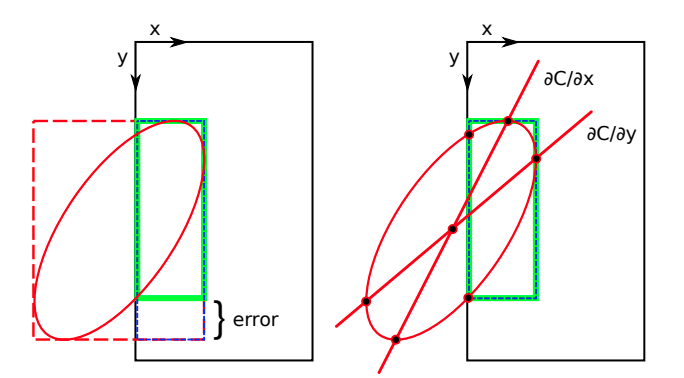
\includegraphics[width=\textwidth, height=0.3\textheight] {Images/bbox_error.png}
    \caption{\centering\textbf{Left}: The dotted red square is the predicted bounding box by the detector. Green square is the required bounding box. Violet is the error. \textbf{Right}: Error is removed through conic extreme x, y parameters\cite{quadric2}}
    \label{fig:bbox_error}
\end{figure}

    \item In the above figure, the black box is the image viewed by the robot and only a part of the conic of the object is visible within the image plane. Normally, the edges of the bounding box is truncated based on the edges of the image plane. And this resulted in the error component depicted by violet color where the object conic is absent.
    \item To reduce this geometric error, the bounding box within image plane is cropped using the conic extreme x and y parameters. For this, 4 points representing extreme points of the conic are selected along with the points that are intersecting between the conic and the 2D bounding box. All the points that lie outside the image plane are removed and from the remaining points within the image plane, the max and min values of x and y are determined which are used to create the accurate green 2D bounding box.
    \item The results of the experiments showed that this feature significantly improved the estimated trajectory and the quadric mapping in terms of reduced trajectory and landmark quality errors.
    \item The previously used error term in Quadric Landmark Factor was an algebraic one. That is, minimizing $\mathbf{q}_{j}^{*}=\operatorname{argmin}_{\mathbf{q}_{j}} \sum_{i k}\left\|\mathbf{l}_{i j k}^{\top} \mathbf{P}_{i} \mathbf{Q}_{\left(\mathbf{q}_{j}\right)}^{*} \mathbf{P}_{i}^{\top} \mathbf{l}_{i j k}\right\|^{2}$. This is replaced by the geometric error proposed by the new sensor model, $\left\|\mathbf{b}_{i j} - \boldsymbol{\beta} _{(x_i,q_j)}\right\|^{2}_{\Lambda_{i j k}}$. Here, ${b}_{i j}$ is the bounding box observed for object j at robot pose i. And $\boldsymbol{\beta} _{(x_i,q_j)} = BBOX(C_{ij})$ is the expected geometrically corrected bounding box for the conic C of the object j observed at pose i. $C = adjoint(C^*) = adjoint(P_i Q^{*}_j P_i^{T})$ where $P_i$ is the camera projection matrix at pose i and $Q^{*}_j$ is the dual quadric representation of the object j.
    \item The 2D object detector used in the experiments is YOLOv3.
    
\subsubsection{Variable Initialization}

\item In the final paper of Quadric SLAM\cite{quadric2}, another initialization method for quadrics are proposed. Using the dual quadric representation of quadric $\pi^{T}Q^{*}\pi = 0$, we can create a linear set of equation which can be solved using SVD if atleast 3 views for the same object quadric is observed. The last column of decomposed matrix V gives the solution for the equation. The translation parameters can be obtained from the last column and the orientation parameters can be obtained from the first three columns of the solved $Q^{*}$ matrix. The size is extracted from the eigen values.\cite{quadric2}
\end{itemize}

\subsection{GTSAM}
\begin{itemize}
\item GTSAM\cite{gtsam} library is used to build the factor graph backend for QuadricSLAM and performs as incremental solvers. The robot pose and the dual quadric matrix are represented as nodes which are the latent variables that needs to be estimated. The pose nodes are constrained by the odometry factors and the pose-quadric nodes are constrained by the bounding box factors.

\begin{figure}[H]
\centering
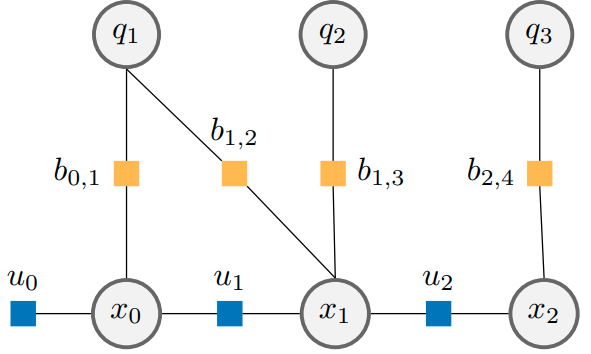
\includegraphics[width=0.6\textwidth, height=0.2\textheight] {Images/factor_graph.png}
\caption{\centering\textbf{Factor Graph of QuadricSLAM}: odometry factors in blue, quadrics bbox factors in yellow \cite{orientation_factor}}
\label{fig:factor_graph}
\end{figure}
\item In the above figure, it can be seen that the quadric $q_1$ is observed from two robot poses $x_0$ and $x_1$. As the same object is observed from different poses, it adds better constraint to optimize the quadric parameters. Actions(in this case robot motion) introduces uncertainty whereas the observations (in this case the bounding boxes of detection) helps to reduce the uncertainty in the pose graph.
\item Another important constraint in factor graph is loop closure constraint. Using the image or quadric features, when the robot detects that its in a pose which was visited at a previous point in time, it can create a loop closure constraint which can help to reduce the overall error in the factor graph. This is also a field of challenge where we need to verify or make sure that the features are qualified enough for a loop closure to avoid false positive loop closure detection which can have a bigger negative effect on the factor graph.
\item The author's of QuadricSLAM, extended the GTSAM functionalities by creating another library called gtsam\_quadrics which handles quadrics related functions.
\item Some of the important functions used in QuadricSLAM are:
\begin{itemize}
    \item gtsam.symbol - used to symbolically represent the robot pose and quadric variables as nodes within the factor graph.
    \item gtsam.noiseModel.Diagonal.Sigmas - can be used to define a noise model which is added into the factor graph when an odometry measurement or observation is used to add a constraint between 2 variables or nodes. It indicates with how much uncertainty, we are adding the measurement to the factor graph.
    \item gtsam\_quadrics.ConstrainedDualQuadric - used to represent the quadric based on the given the input parameters like rotation, translation, radii matrixes as it has different constructors.
    \item gtsam.NonlinearFactorGraph - Used to initialize a factor graph onto which the robot pose and quadrics are added as latent variables along with the odometry and bounding box measurements as factors with an assosciated noise model.
    \item gtsam.Cal3\_S2 - to generate calibration matrix
    \item gtsam.Pose3 - create a 3D pose of rotation and translation matrix based on the input provided.
    \item gtsam.Rot3 - create a 3D rotational matrix.
    \item gtsam.PriorFactorPose3 - to generate the initial robot pose with a prior noise model which is added to the factor graph.
    \item gtsam.BetweenFactorPose3 - to add the odometry measurement factor between two robot poses with a odometry noise model which is added to the factor graph.
    \item gtsam\_quadrics.BoundingBoxFactor - to add the bounding box observation as a factor between a robot pose and a quadric which is added to the factor graph. Bounding box noise is also assosciated with the function.
    \item gtsam\_quadrics.QuadricCamera.project - given a dual quadric matrix and robot pose, it will generate the 2D view(conic) of the quadric in the image plane from which using the function bounds(), we can obtain the 2D bounding box virtually.
    \item gtsam.LevenbergMarquardtOptimizer - Given the factor graph and a initial estimate for the robot poses and quadric latent variables, a non-linear optimization is applied on the graph to get the results.


    
\end{itemize}

\item It can be seen that there is a noise model attached to every odometry, observation and prior measurement factor. This creates the uncertainty region for adjusting the edges between the nodes during bundle adjustment. If the noise model is set to 0, it means the measurement is taken with 100\% accuracy and then the node(in this case, the camera pose or the object pose) will be fixed or immovable.
\end{itemize}

\subsection{Code Explanation}
\begin{itemize}

\subsubsection{Overall Framework}
\begin{figure}[H]
\centering
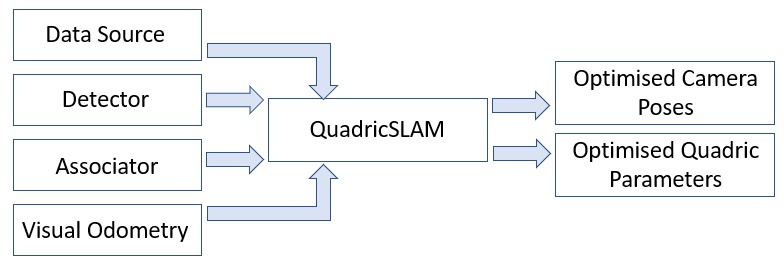
\includegraphics[width=\textwidth] {Images/QuadricSLAM.jpeg}
\caption{\centering QuadricSLAM framework}
\label{fig:framework}
\end{figure}

\item The above figure depicts the general functional framework of QuadricSLAM. QuadricSLAM is implemented as a class which takes in the class objects of data source, detector, associator and visual odometry. And what we get out of QuadricSLAM is the optimised camera poses and quadric parameters which can be used to create the map. Each component is explained below.

\subsubsection{Data source}
\begin{figure}[H]
\centering
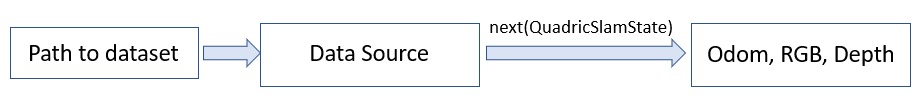
\includegraphics[width=\textwidth] {Images/data_source.jpeg}
\caption{\centering Data source}
\label{fig:data_source}
\end{figure}

\item Used to either access an available dataset(acts as a dataloader) or provide the live data to the QuadricSLAM algorithm. The data include odometry, RGB image and depth image. These data is retrieved by QuadricSLAM by calling the next() function of data source.
\item The odometry should be converted from quaternion or transformation matrix format to SE3() pose representation in spatial math.
\item Datasource also maintains an internal counter to step through each data in time and also checks for data read completely or not.
\item Depthscaling factor and RGB calibration parameters are also stored here. Images are calibrated before passing into the QuadricSLAM.
\item If using a live data, then the configuration of the data source can be defined in the init() function. If using an available dataset, then the path to the dataset is to be passed into here.

\subsubsection{Detector}
\begin{figure}[H]
\centering
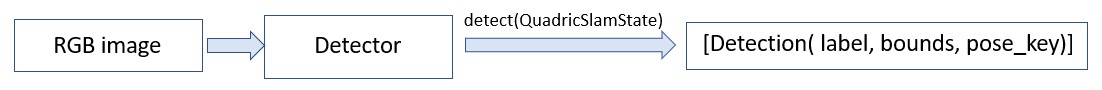
\includegraphics[width=\textwidth] {Images/Detector.jpeg}
\caption{\centering Detector}
\label{fig:detector}
\end{figure}

\item Used for detecting objects in each RGB image frame. The detect() function outputs the list with elements of object type Detection which contains label of the object, list of 4 values of the bounding box(x,y of top-left and bottom-right corners) and the pose\_key which indicates at which pose number the current detection is made.
\item The default detector used here is the detectron2 Faster-RCNN. A pretrained model on certain labels is used here. Only those objects are detected.
\item In the experiments which we are going to perform on BOP dataset, we are going to avoid the usage of a detector and instead provide the bounding box directly available from the dataset. This will help us to evaluate the performance of QuadricSLAM given the noise from the bounding box is kept minimum.

\subsubsection{Associator}
\begin{figure}[H]
\centering
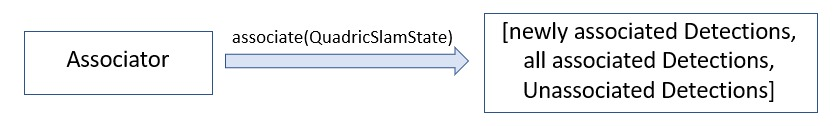
\includegraphics[width=\textwidth] {Images/associator.jpeg}
\caption{\centering Associator}
\label{fig:associator}
\end{figure}

\item Data Associator takes the detections made in the current state and all previously unassosciated detections and used it to compare with previously assosciated detections to decide whether to match the unassosciated detection with a previously assosciated detection(same quadric key to both detection) or to treat the detection as a new object(new quadric key to the detection).
\item Basically, it decides whether a detection should be given an existing quadric key or create a new quadric key for it.
\item The decision is based on the Intersection Over Union(IOU) value between the detection and an existing quadric. With respect to the current robot pose, all the existing quadrics within the factor graph is projected in 2D plane as a enclosing bounding box. For each current detection bounding box, we are comparing its overlap with each bounding box generated within the map of QuadricSLAM. If the overlap is below a certain threshold, then treated as a new object with a new quadric key. Otherwise, assosciated to an existing object with the quadric key of the overlapping quadric.
\item In the init() function, we can specify threshold above which an assosciation should be made.
\item The associate() function outputs the list of the newly associated detections(objects for which a new quadric has been created in the current step), updated list of associated detections(all objects that has been assosciated with a quadric key), updated list of unassociated detections(objects that doesn't have a quadric key - usually passed as an empty list).

\subsubsection{Visual Odometry}
\begin{figure}[H]
\centering
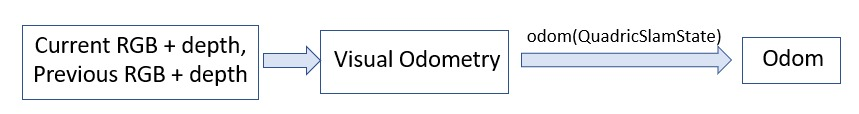
\includegraphics[width=\textwidth] {Images/visual_odometry.jpeg}
\caption{\centering Visual Odometry}
\label{fig:visual_odometry}
\end{figure}

\item Could be used to generate the odometry from current and previous RGBD image. Usefull when no odometry information is available.
\item Here, RgbdOdometry from CV2 library is being used. The current and previous RGB images are converted intro gray scale and provided as input along with their depth images to compute the odometry.
\item odom() function returns the odometry value.
\item Other visual odometry approaches suggested by the authors are ORB-SLAM2 with loop closure disabled or Kimera VIO(Visual Inertial Odometry) to get a less noisy odometry value.
\end{itemize}

\subsubsection{Main code}
\begin{itemize}
\item There are two ways to initialize a quadric. initialise\_quadric\_ray\_intersection() and \newline initialise\_quadric\_from\_depth().
\item In initialise\_quadric\_ray\_intersection(), the translation and rotation of the poses at which a particular object is seen is used to project rays into 3D space and using least squares method to find the closet converging point which is a good approximation of the quadric centroid. The initial orientation and size of the quadric is random. In the code, the size is set to (1, 1, 0.1).
\item In initialise\_quadric\_from\_depth(), the quadric can be initialized from a single view or image. To estimate centroid, the z coordinate is calculated as the mean of the depth of points within the bounding box of detection. x and y coordinate are calculated as a calibrated value representing the centre point of the bounding box. The x,y radii of the quadric is calculated as a calibrated value of the height and width of the bounding box. The z radii is assumed to be a predefined object depth of 0.1. The orientation of the quadric can be estimated using the rotation, translation of the camera pose and the quadric centroid through gtsam.PinholeCameraCal3\_S2.Lookat() function.
\item There are two modes of optimization. Optimization in a batch or in an incremental way. If its set to true, then the optimization of the unknown variables occur only at the end of processing all the images. If false, then the optimization runs along with each detection step.
\item There are 3 noise models used in this application. One for the prior noise which is added along with the initial pose of the robot. Another one for odometry measurement noise which is added to the constraint between two robot pose variables. Third one for bounding box noise which is added for the constraint between a robot pose and the observation measurement which is a bounding box. This noise is due to the instability of bounding box being generated for an object which is evident for small objects.


\begin{figure}[H]
\centering
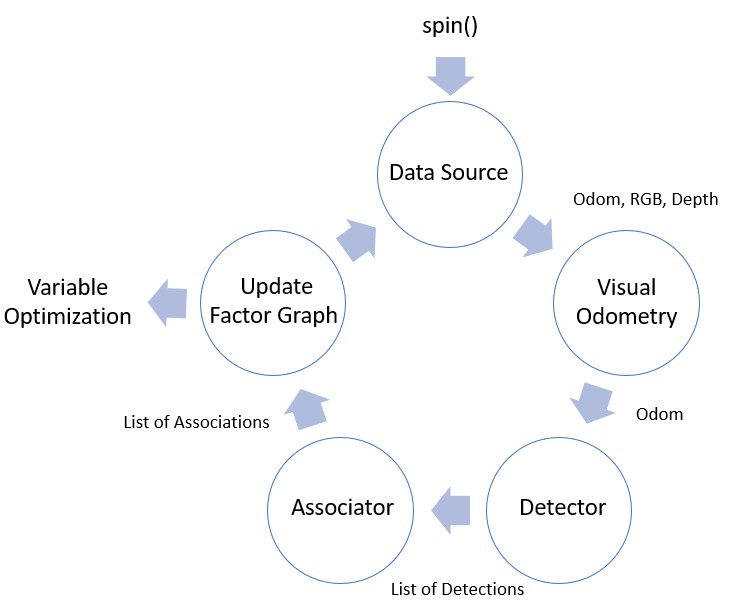
\includegraphics[width=\textwidth] {Images/spin.jpeg}
\caption{\centering spin() function of QuadricSLAM}
\label{fig:spin}
\end{figure}

\item The above figure 6 depicts the main operation of the QuadricSLAM which is the spin() function.
\item The next() function of the datasource returns the current odom, RGB and depth.
\item If there is no odom data, a visual odometry method could be used to generate the odom data.
\item The detector takes in current RGB image and outputs a list of detections with information about the label, bounds and pose\_key for each detected object. detect() function is used.
\item The associator takes these detections and use IOU method to identify whether its an new object or an existing object in the graph. All the associations and unassociations are outputed by the associate() function.
\item Based on the new pose and quadric information, the non linear graph is updated.
\item This cycle of process continues until the dataset is completely processed.
\item Based on the optimization batch setting that have been set, the unknown variables are either optimized at the end of processing all the dataset or done in an incremental fashion during each cycle.
\item The values to be recorded after running the algorithm are state.estimates - which has the initial guess of the quadrics and the poses onto which the non-linear graph perform optimisation and state.labels - which has the actual label for the quadric key which we can use for evaluation purposes. Since, objects of same class appears multiple times within the graph, we cannot just use the actual label within the graph. So they are represented by a random number and this is stored in the state.labels.
\end{itemize}

\subsection{Key insights}
\begin{itemize}
\begin{figure}[H]
\centering
\begin{minipage}{.5\textwidth}
  \centering
  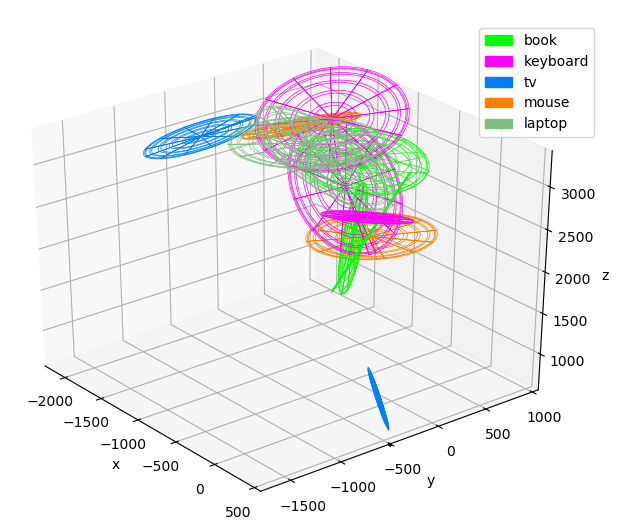
\includegraphics[width=\textwidth]{Images/batch_14_2bookNaN.png}
  \captionof{figure}{Batch optimization}
  \label{fig:batch_14_2bookNaN}
\end{minipage}%
\begin{minipage}{.5\textwidth}
  \centering
  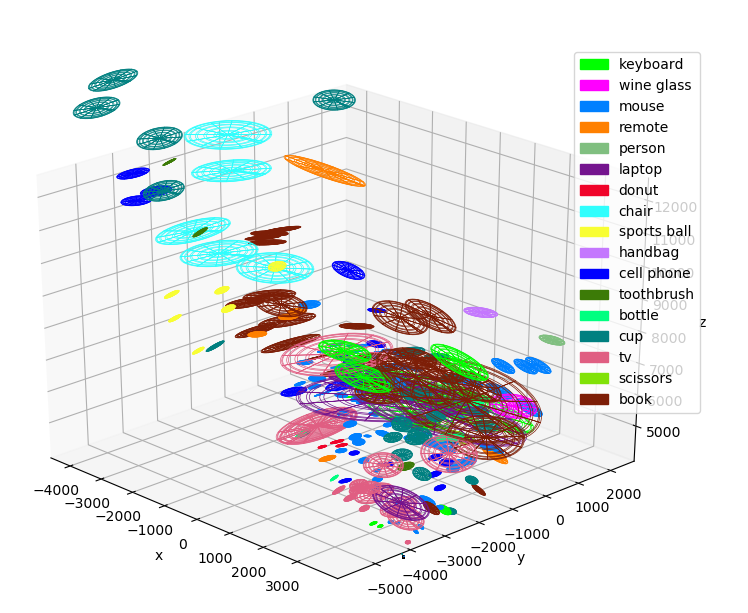
\includegraphics[width=\textwidth]{Images/incremental_236.png}
  \captionof{figure}{Incremental optimization}
  \label{fig:incremental_236}
\end{minipage}
\end{figure}

\item The above plots represent the quadric representation of the freiburg1\_desk scene of TUM RGBD dataset. In figure \ref{fig:batch_14_2bookNaN}, the optimization of the factor graph is performed only at the end of reading the entire dataset(batch optimization). And the initial guess of the odometry value is the same as that of the provided ground truth odometry as we didn't used any explicit odometry estimation algorithm here. Because of that, the data association in each step of the data performed well in associating quadrics that belong together and thus generating 14 detected objects or quadrics in the end. Whereas in incremental optimization approach (figure \ref{fig:incremental_236}), at each step, based on the initialized quadric from a single detection and the ground truth odometry, the factor graph is optimized. Thus the actual ground truth odometry is pulled to a wrong position to compensate for the noisy quadric detected. And this error accumulates over each time step and each detections of the same object in each data step appears at different locations in environment. This is the data assosciation problem in QuadricSLAM that leads to duplication. Thus 236 quadrics are generated in the end as most of the detections of the same object couldn't be assosciated together.
\item Another observation is that, since a single detection is used to generate a quadric, the uncertain predictions of the detector will generate some non existing objects due to the wrong label prediction. In the figure \ref{fig:incremental_236}, objects like person, sports ball were not present in the environment. There should have been a counter to detect the number of times a particular label appears for a quadric and the final label should the most occurring one. This is possible only if the data assosciation problem is solved.

\subsubsection{Benefits}
\begin{itemize}
\item Geometric SLAM approaches utilised features like ORB\cite{orbslam}, lines\cite{linesegment}, planes\cite{infiniteplanes} to represent the environment. But they lacked the semantic information for these geometrical features. And these features were used only to estimate the robot pose and create a dense point cloud of the environment. Whereas in Quadric SLAM, the knowledge of semantic label of the geometric represented as a quadric can help in loop closure and creation of a semantically enriched object-oriented map.
\item As compared to SLAM++\cite{slam++} approach where prior knowledge of CAD models are used to represent the objects when they are detected, the Quadric SLAM doesn't require priors. For example, there can be different variations of chair and in SLAM++, it would be represented using the same CAD model of chair which can affect the mapping accuracy. In Quadric SLAM, the position, size and orientation could be accurately estimated from multiple views of the chairs thereby producing quadrics of different parameters for each type of chair.
\item In SemanticFusion\cite{semanticfusion}, each point in the point cloud is having a label and the 3d object reconstruction from the dense point cloud is performed as a post-processing step. In the proposed Quadric SLAM approach, the object representation as quadrics(mapping) is performed in an online fashion. Also, the sparse representations can help in easier storage of the map. For example, the 9 parameters of the dual quadric could be saved as a XML file.

\end{itemize}

\subsubsection{Challenges}







\end{itemize}
    \section{OA-SLAM}

    \subsection{Related works}
    \subsubsection{4.2.1.1 ORB-SLAM2}
    \subsubsection{4.2.1.2 Structure Aware SLAM using Quadrics and Planes\cite{StructureAS}}
    \begin{itemize}
    \item As a continuation of quadricSLAM, Sünderhauf et. al. also looked into extracting planes from the environment which can act as an extra constraint combined with the feature points within the factor graph\cite{StructureAS}.
    \item This concept of infinite planes was first introduced into factor graphs as a least-squares optimization problem in the paper by Kaess\cite{infiniteplanes}. And later, Taguchi et. al. presented a SLAM method where a combination of planes and points can be used to register 3D data, since a single plane can be used to replace a lot of inlier 3D points which can help in faster computations and compact representations.\cite{infpla2}
    \item In this work, planes are also considered as an important feature which is the most common feature occurring in indoor environments. A plane can represent a big region of the environment, especially in cases where there are very few objects within the environment to be mapped and used as anchors.
    \item These planes can be used to create three additional constraints. Constrain between the points lying on the plane and the plane parameters. Constrain between the object and the supporting plane parameters. Constrain between two planes.
    \item The following section explains about the mathematics behind quadric and plane representations along with how the constraints can be added to the factor graph as a non-linear least squares problem. The section is a summarized version of the content in section 3 of the "Structure Aware SLAM using Quadrics and Planes" paper\cite{StructureAS}.
    \item From the previous section on QuadricSLAM, we have seen that the closed-form equation of quadric with tangential planes is given by $\pi^{T}Q^{*}\pi = 0$ where $Q^{*}$ is called as dual quadric representation. There are 9 unique elements within this symmetric matrix that needs to be estimated through error minimization. So the error vector generated is 9 dimensions.
\begin{equation}
{
\begin{aligned}
\mathbf{Q}^{*}=\mathbf{T}_{Q} \mathbf{Q}_{c}^{*} \mathbf{T}_{Q}^{T}=\left[\begin{array}{cc}
\mathbf{R} & \mathbf{t} \\
\mathbf{0}^{T} & 1
\end{array}\right]\left[\begin{array}{cccc}
a^2 & 0 & 0 & 0\\
0 & b^2 & 0 & 0\\
0 & 0 & c^2 & 0\\
0 & 0 & 0 & -1
\end{array}\right]\left[\begin{array}{cc}
\mathbf{R}^{T} & \mathbf{0} \\
\mathbf{t}^{T} & 1
\end{array}\right] \quad 
\end{aligned}
} \label{eq:dual_quad}
\end{equation}
\item Since we are fixing the quadric to be ellipsoid in this application, the dual quadric representation $Q^{*}$ could be written as  \ref{eq:dual_quad}. ${T}_{Q}$ is the transformation matrix that transforms the ellipsoid from its origin by rotating and translating it. ${Q}_{c}^{*}$ is the ellipsoid located at the origin with radius a,b and c. The last element of ${Q}_{c}^{*}$ is made -1 to represent the dual quadric matrix as an ellipsoidal equation.

\begin{equation}
{
\begin{aligned}
\mathbf{Q}^{*}=\mathbf{T}_{Q} \mathbf{Q}_{c}^{*} \mathbf{T}_{Q}^{T}=\left[\begin{array}{cc}
\mathbf{R} & \mathbf{t} \\
\mathbf{0}^{T} & 1
\end{array}\right]\left[\begin{array}{cc}
\mathbf{L L}^{T} & \mathbf{0} \\
\mathbf{0} & -1
\end{array}\right]\left[\begin{array}{cc}
\mathbf{R}^{T} & \mathbf{0} \\
\mathbf{t}^{T} & 1
\end{array}\right] \quad \text { where } \quad \mathbf{L}=\left[\begin{array}{lll}
a & 0 & 0 \\
0 & b & 0 \\
0 & 0 & c
\end{array}\right]
\end{aligned}
} \label{eq:dual_quad_upd}
\end{equation}

\item Further, to make sure that the first 3 diagonal elements of the ${Q}_{c}^{*}$ matrix are positive eigen values during optimization process in factor graphs, the equation \ref{eq:dual_quad} is updated to \ref{eq:dual_quad_upd} so that it guarantees positive values.
\item Now updation of ${Q}^{*}$ means updating T and L where T is the transformation matrix of 6 parameters(3 rotation and 3 translation) and L is a diagonal matrix with 3 parameters(a, b, c scale parameters). Thus the 9 dimension error can be split into 6-dim and 3-dim errors for efficient computation.

\begin{equation}
{
\begin{aligned}
\mathbf{Q}^{*} \oplus \Delta \mathbf{Q}^{*}=(\mathbf{T}, \mathbf{L}) \oplus(\Delta \mathbf{T}, \Delta \mathbf{L})=(\mathbf{T} \cdot \Delta \mathbf{T}, \mathbf{L}+\Delta \mathbf{L})
\end{aligned}
} \label{eq:param_upd}
\end{equation}

\item The updation of quadric parameters in ${Q}^{*}$ can be simplified as in equation \ref{eq:param_upd}. The $\Delta$ values indicate the update value. In the case of L, the updation operation is addition based on the first 3 values of the 9 dim error vector and in case of T, it needs to perform the transformation operation for the updation based on the last 6 values of the 9 dim error vector.
\item This representation of ${Q}^{*}$ in terms of T and L also helps to add initial prior information about the properties of the object into the factor graph. The size info can be initialized in L matrix and the rotation and translation info can be initialized in T matrix.

\item Next, we have to represent the planes in mathematical form. Inspired by the work on infinite planes by Kaees\cite{infiniteplanes}, an infinite plane is represented by normalised homogeneous coordinates $\mathbf{\pi}=
{\begin{bmatrix}
    a & b & c & d
\end{bmatrix}}^{T}
$ to have a compact representation. n is the normal vector 
$\mathbf{n}=
{\begin{bmatrix}
    a & b & c
\end{bmatrix}}^{T}
$ and d is the distance to the origin. This normal vector can be optimised using the rotation matrix algebra.

\begin{figure}[H]
\centering
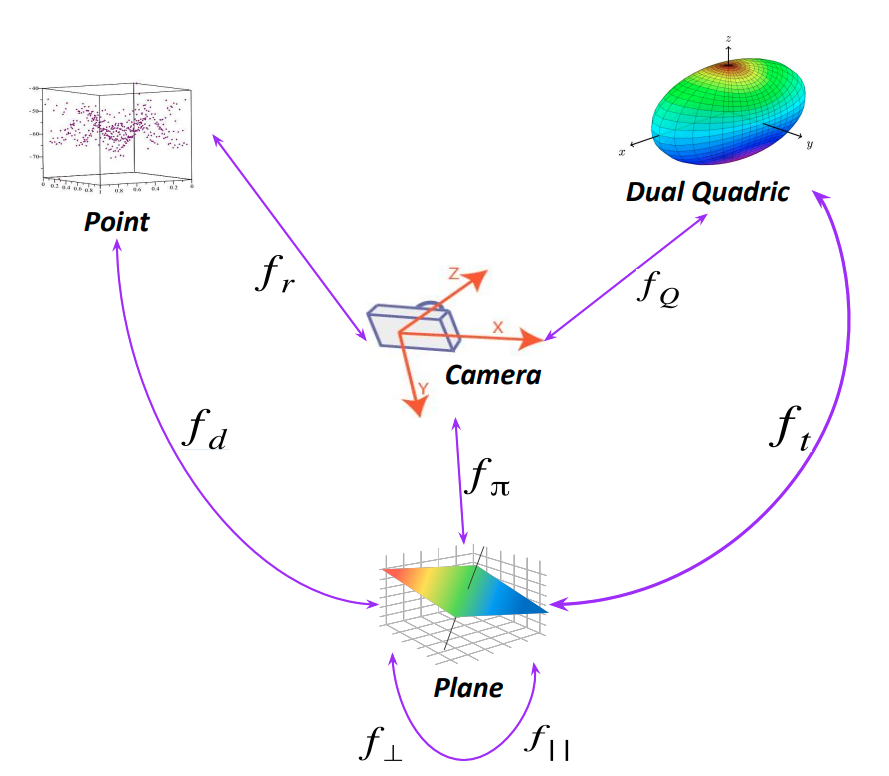
\includegraphics[width=\textwidth] {Images/struc_awa_slam.png}
\caption{\centering Factor graph containing points, planes and objects \cite{StructureAS}}
\label{fig:struc_awa_slam.png}
\end{figure}

\item The above figure \ref{fig:struc_awa_slam.png} shows the factor graph containing the nodes/ variables representing camera pose, 3D points, quadric parameters, plane parameters that need to be estimated and the connecting edges which represent 7 different types of factor constraints($f_{r}, f_{Q}, f_{\pi}, f_{d}, f_{t}, f_{\|}, f_{\perp}$).

\item \textbf{1. Observation of points($f_{r}$): } The 3D points observed by the camera at a particular pose is to be registered within the factor graph. The equation tries to minimize the reprojection error.

\begin{equation}
{
\begin{aligned}
f_{r}\left(\mathbf{x}_{w}, \mathbf{T}_{c}^{w}\right)=\left\|\mathbf{u}_{c}-\Pi\left(\mathbf{x}_{w}, \mathbf{T}_{c}^{w}\right)\right\|_{\mathbf{\Sigma}_{r}}
\end{aligned}
} \label{eq:point_factor}
\end{equation}

In the above equation \ref{eq:point_factor}, $x_{w}$ represents the 3d point in world coordinates, $T_{c}^{w}$ represents the transformation matrix of the pose of the camera w.r.t the world that can map the observed point in the current pose c to the world coordinate system. The error is calculated between the pixel location of the point $u_{c}$ in the current pose $c$ and the reprojected point from the world coordinate into the camera frame using the function $\Pi()$. The error function is the Mahalanobis norm $\mathbf{x}^{T} \boldsymbol{\Sigma}^{-1} \mathbf{x}$ where $\Sigma$ is the uncertainty matrix associated with the factor. Mahalanobis norm takes the covariance structure of the data into consideration while reducing the reprojection error where the distance to the distribution is utilized instead of the distance to a single point as in the euclidean norm.

\item \textbf{2. Observation of objects($f_{Q}$): } The objects in this case are the ellipsoids. So need to reduce the reprojection error between the conic of the viewed object and the reprojected conic from the ellipsoid in the world cordinates at a particular camera pose $c$. More details on the conic equation formation in mentioned in the above section on QuadricSLAM.

\begin{equation}
{
\begin{aligned}
f_{Q}\left(\mathbf{Q}^{*}, \mathbf{T}_{\mathbf{c}}^{\mathbf{w}}\right)=\left\|\mathbf{C}^{*}-\mathbf{C}_{\mathbf{o b s}}^{*}\right\|_{\mathbf{F}}=\sqrt{\mathbf{T r}\left(\left(\mathbf{C}^{*}-\mathbf{C}_{\mathrm{obs}}^{*}\right)\left(\mathbf{C}^{*}-\mathbf{C}_{\mathrm{obs}}^{*}\right)^{\mathbf{T}}\right)}
\end{aligned}
} \label{eq:object_factor}
\end{equation}

In the above equation \ref{eq:object_factor}, the norm being used is Frobenius norm. It is measuring the magnitude of the matrix or in other words the root of summed squares of the elements of the matrix. Can be used to check for residuals. Since we are trying to reduce the reprojection error, ideally the value should be 0 or close to 0.

\item \textbf{3. Observation of planes($f_{\pi}$): } The distance between observed plane $\pi_{obs}$ at a particular camera pose $c$ and the plane parameters in the world coordinate $\pi$ projected into the camera frame is minimized. Since the normal vector $n$ is used to describe the plane, the distance measured is based on the rotational distance in rotation space between the normal vector for $\pi$ and $\pi_{obs}$ which is explained in the work by Kaess\cite{infiniteplanes}.

\begin{equation}
{
\begin{aligned}
f_{\pi}\left(\pi, \mathbf{T}_{\mathbf{c}}^{\mathbf{w}}\right)=\left\|d\left(\mathbf{T}_{c}^{w-T} \pi, \pi_{o b s}\right)\right\|_{\Sigma}^{2}
\end{aligned}
} \label{eq:plane_factor}
\end{equation}

\item \textbf{4. Point-plane constraints($f_{d}$): } If there is a certainty that a point lies on a plane, then the constraint between the point and the plane can be established as minimizing the orthogonal distance between the normal vector $n$ representing the plane and a vector formed between the point $x$ and a random point $x_o$ on the plane.

\begin{equation}
{
\begin{aligned}
f_{d}(x, \pi)=\left\|\mathbf{n}^{T}\left(\mathbf{x}-\mathbf{x}_{o}\right)\right\|_{\sigma}^{2}
\end{aligned}
} \label{eq:point_plane_factor}
\end{equation}

In the above equation \ref{eq:point_plane_factor}, the dot product between the two vectors is taken. The normal vector $n$ is perpendicular to the plane surface and if the point $x$ is on the plane surface, then the vector connecting $x$ and $x_o$ would be perpendicular to the normal vector and the dot product would be 0.

\item \textbf{5. Supporting plane constraints($f_{d}$): } In the real world, all the objects on the floor or on the walls are supported by a plane. For example, a clock is supported by a wall plane and a computer is supported by a table plane. This knowledge is exploited to create a constraint between the object and the supporting plane. The same equation which was used to define dual quadrics, i.e. a quadric is enclosed by tangential planes is used here also.

\begin{equation}
{
\begin{aligned}
f_{t}\left(\pi, \mathbf{Q}^{*}\right)=\left\|\pi^{T} \mathbf{Q}^{*} \pi\right\|_{\sigma}^{2}
\end{aligned}
} \label{eq:support_plane_factor}
\end{equation}


\item \textbf{6. Plane-plane constraints($f_{\|}, f_{\perp}$): } Based on the Manhattan assumption, 2 planes can either be perpendicular or parallel.

\begin{equation}
{
\begin{aligned}
\begin{gathered}
f_{\|}\left(\pi_{1}, \pi_{2}\right)=\left\|\left|\mathbf{n}_{1}^{\top} \mathbf{n}_{2}\right|-1\right\|_{\sigma}^{2} \quad \text { for parallel planes } \\
f_{\perp}\left(\pi_{1}, \pi_{2}\right)=\left\|\mathbf{n}_{1}^{\top} \mathbf{n}_{2}\right\|_{\sigma}^{2} \quad \text { for perpendicular planes }
\end{gathered}
\end{aligned}
} \label{eq:plane_plane_factor}
\end{equation}

In the above equation \ref{eq:plane_plane_factor}, the dot product between the normal vectors of plane 1 and 2 is taken. In case of parallel planes, the dot product would be 1 and the error term would be 1-1=0 and in the case of perpendicular planes, the dot product would be 0.

\begin{figure}[H]
\centering
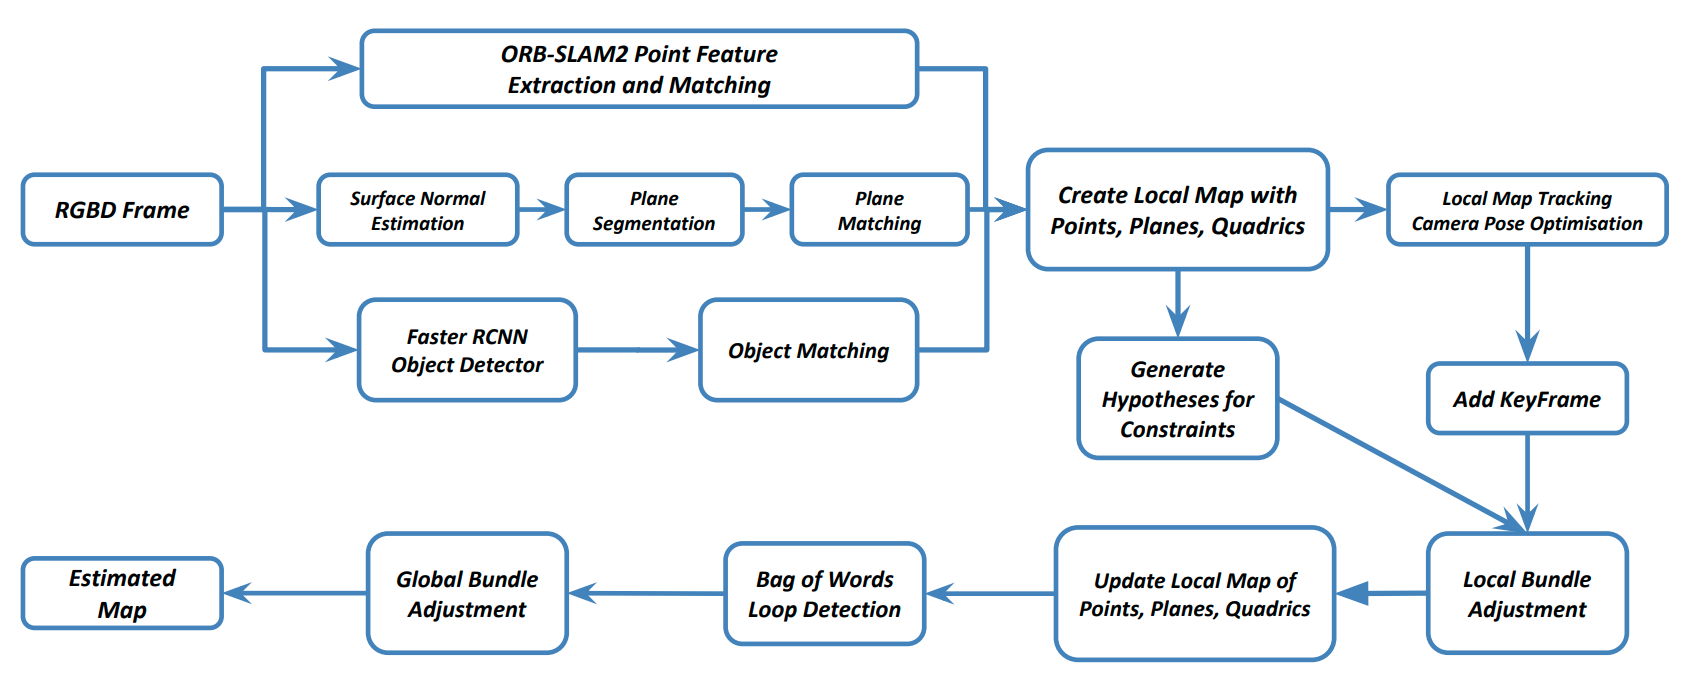
\includegraphics[width=\textwidth] {Images/slam_pipeline.png}
\caption{\centering SLAM pipeline \cite{StructureAS}}
\label{fig:slam_pipeline.png}
\end{figure}

\item The above figure \ref{fig:slam_pipeline.png} represents the internal pipeline of the slam. This architecture is based on ORB-SLAM except for the fact that the plane and object detection is added in parallel to the point detection at the input side of the pipeline. The optimization step happens in an incremental fashion whenever a new keyframe is added along with its observations (basically an input image and the observed objects, planes and points). Loop closures are detected based on ORB feature matching using the bag of words method as in ORB-SLAM. The input is an RGBD image instead of an RGB image in ORB SLAM for the purpose of plane detection and object quadric initialization. The authors also plan to remove the use of RGBD images and use monocular RGB images in future work to perform depth estimation and semantic segmentation on single images.
\item \textbf{1. Observation of points: } This is the same as in the ORB-SLAM. Unique ORB features are identified, tracked and matched(data-assosciation) between images. The depth initialization for these points can be made available from the depth channel if an RGBD image is provided as input or can estimate the depth between consecutive RGB images.
\item \textbf{2. Observation of objects: } A pre-trained Faster-RCNN is used to generate the bounding boxes through object detection. The conic is fitted into the bounding box as explained in the previous section on QuadricSLAM. To deal with noisy detections, the object is initialized only if it is having a confidence of above 95\% for a class label. Also to solve the data association problem if multiple copies of the same object are present, a nearest neighbour approach is used to find whether they are 2 separate objects or inconsistent detection of the same object.
\item \textbf{3. Observation of planes: } Usually planes are detected using RANSAC which not be sufficient to meet the runtime requirements in SLAM to perform online operations. Also we need a finite boundary for the planes instead of infinite plane representation.
\item Trevor et.al \cite{effplaneseg} utilizes the availability of organized point clouds(2D image with depth channel as compared to LIDAR point clouds) to perform segmentation which can reduce the time taken for neighbourhood searching step in unorganized point clouds. Each pixel is assigned a label and 2 pixels can have the same label if they are similar. In the first pass, the first row and first column of the image point cloud are assigned labels based on their similarity with immediate neighbours. After that, for each other pixel, its top and left neighbours are compared for similarity. If similarities are detected, then in the second pass of the algorithm, the labels are merged. To detect planar surfaces from these point clouds, for each point belonging to labels having a large surface(corresponding to floor, wall, ceiling), a surface normal is computed to represent the plane equation. The fourth plane component d is also computed using the dot product of the surface normal and the point's coordinate. Then the angular distance(dot product) between the surface normals and the L1 norm of the d distance parameters of the 2 points as the similarity factor to identify points belonging to a connected plane based on certain thresholds. Since smooth curved surfaces are also getting detected through this method, a max allowable curvature threshold is also set. To identify large surfaces, the min inlier point threshold is set. Later a plane refinement step is also performed to get a less noisy boundary by taking in unsegmented boundary pixels also. The authors also mention that the colour could be also used as a similarity measure by comparing in the Euclidean space.
\item For data association in the factor graph, all planes are considered as the number of planes in an environment is assumed to be sparse and also the viewpoint change of the planes between the subsequent image frames is assumed to be less. The data association can be performed by comparing the normal vectors and distance parameters of the plane equations.

\item \textbf{4. Point-plane constraints: } After performing the plane detection, the inlier points are detected by comparing the distance of the point from the camera with a threshold value. This is because the farther the point is from the camera, then the depth will have higher uncertainty. If it satisfies the inlier condition, then it is added to the factor graph as a point-plane constraint.

\item \textbf{5. Supporting plane constraints: } The supporting infinite plane for the object is identified by comparing the orthogonal distance of the centroid of the object quadric with the plane. If it is less than a threshold defined by $max(20cm, a, b, c)$, then the object is supported by the plane. a, b, c is the radius of the ellipsoid and hence the threshold is dependent on the size of the quadric.

\item \textbf{6. Plane-plane constraints: } For establishing plane-to-plane constraints, every plane is taken into consideration(due to the sparsity of the planes) and a parallel or perpendicular constraint is established if the angle difference between the normals of the plane is within a certain window range. The uncertainty for this constraint is set to high so that the factor graph won't force them to be always perpendicular or parallel but act as a good prior for relative orientation between the planes.


\item In the evaluation part, a qualitative comparison is performed as we don't have the ground truth mapping data available for the TUM-RGBD dataset. In quantitative comparison, only RMSE Absolute Trajectory Error (ATE) is estimated. The qualitative comparison is performed because the real world cannot be exactly and semantically mapped for the ground truth. So the best solution is to create a virtual environment in simulators like Gazebo or frameworks like BenchBot(\href{https://github.com/qcr/benchbot}{link}).

\end{itemize}

    \subsection{Summary}
    \begin{itemize}
\item The OA-SLAM\cite{oaslam} stands for Object Aided SLAM which utilizes the objects as a key feature for aiding mapping and camera relocalization. It is an improved version of quadric SLAM where the feature points within the environment are also mapped along with the quadric shapes(ellipsoids, cuboids) to improve object tracking and pose recovery in case of tracking failures during sudden motions.
\item This method is built on top of ORB-SLAM2. ORB-SLAM utilizes visual bag-of-words keypoint descriptors to compare the ORB features in the current scene with the reference map of the environment. The disadvantage is its restricted invariance to viewpoint changes which makes it difficult to localize when some landmark points are not visible in the current image frame.
\item The low-level landmark points are combined with the quadrics of the object generated through object detection methods to form high-level landmarks where objects can be used as anchors for mapping and localization. This can help to improve the viewpoint invariance.
\item Even though the representation of the environment with the help of key points helped in efficient computations in ORB-SLAM, it lacked the semantic meaning which could be useful for relocalization in a dynamic environment. 
\end{itemize}

\begin{itemize}
    \item Previous works on sparse, dense and semi dense
    \item Previous work on quadric parameters estimation from bounding boxes of object detections.
    \item Previous work on initial quadric parameter estimation.
    \item Previous work on camera pose estimation utilizing objects using a pre-built object map.
    \item Previous work on semantic segmentation on point cloud as a post-processing step to generate dense object maps. Cannot be used for localization as its a post-process step.
    \item Previous work of QuadricSLAM\cite{quadric2} was mentioned and the disadvantage was the assumption of the data association is solved.
    \item Previous works on fitting a predefined CAD model onto the object once it is detected.
    \item Previous work focuses on dense point cloud mapping of objects whereas we focus on an approximate representation of the object properties in terms of position, size and orientation that could be used in most of the applications except where manipulation of the object is needed.
    
\end{itemize}

\subsection{Code Explanation}
\subsubsection{Pangolin}
\subsubsection{Ceres}

\subsection{Key insights}
\subsubsection{Benefits}
\begin{itemize}
    \item Useful in AR applications where the objects and points can be used to relocalize the camera pose when the camera tracking fails.
    \item Virtual objects can be placed in the real world over the objects identified during the SLAM.
    \item The proposed approach require only RGB camera instead of RGB-D camera which is very helpful in deployment in devices like mobile phones.
    \item The object mapping and camera pose is estimated on real time.
\end{itemize}
\subsubsection{Challenges}


\section{Comparative Evaluation of SLAM pipelines}

\begin{figure}[H]
\centering
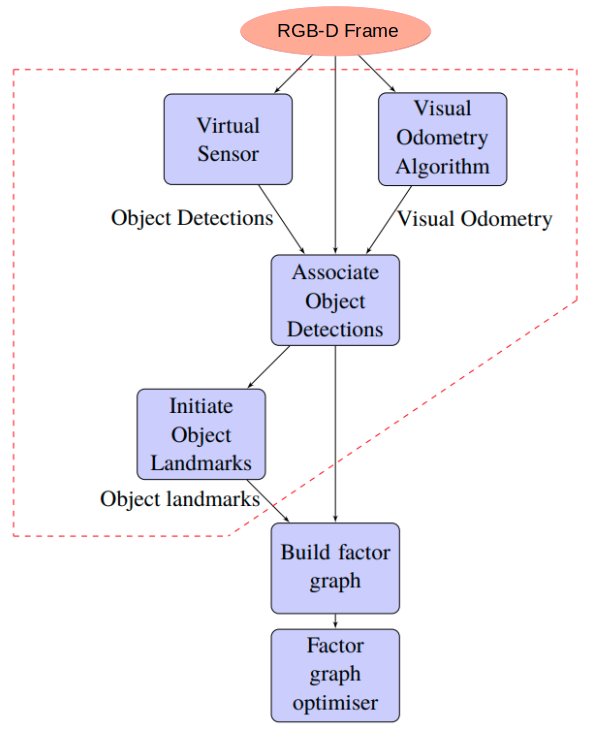
\includegraphics[scale=0.35] {Images/qslam.png}
\caption{\centering Quadric SLAM pipeline \cite{dataassosciation}}
\label{fig:qslam.png}
\end{figure}

\begin{figure}[H]
\centering
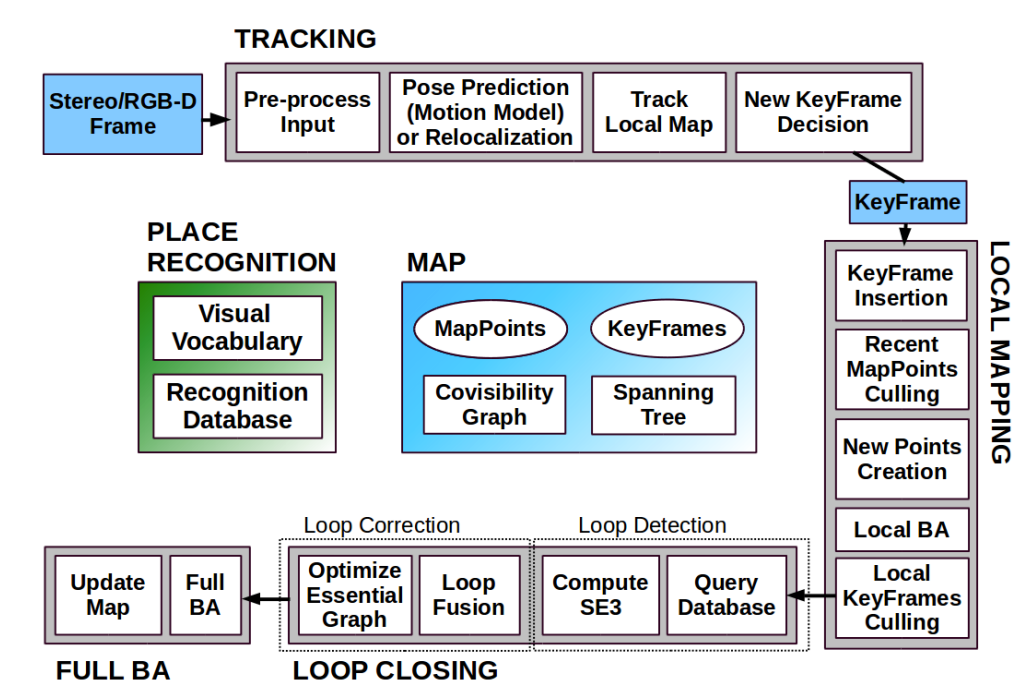
\includegraphics[scale=0.3] {Images/orb_slam2.png}
\caption{\centering ORB-SLAM2 pipeline \cite{orbslam2}}
\label{fig:orb_slam2.png}
\end{figure}

\begin{figure}[H]
\centering
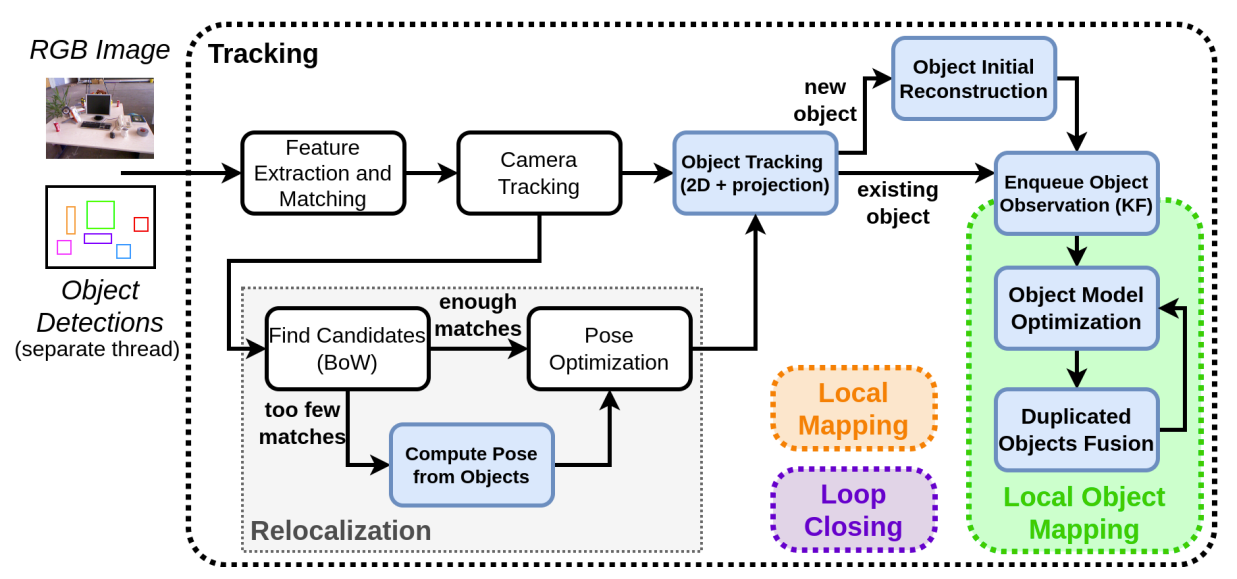
\includegraphics[scale=0.3] {Images/oa_slam.png}
\caption{\centering OA-SLAM pipeline \cite{oaslam}}
\label{fig:oa_slam.png}
\end{figure}

\begin{figure}[H]
\centering
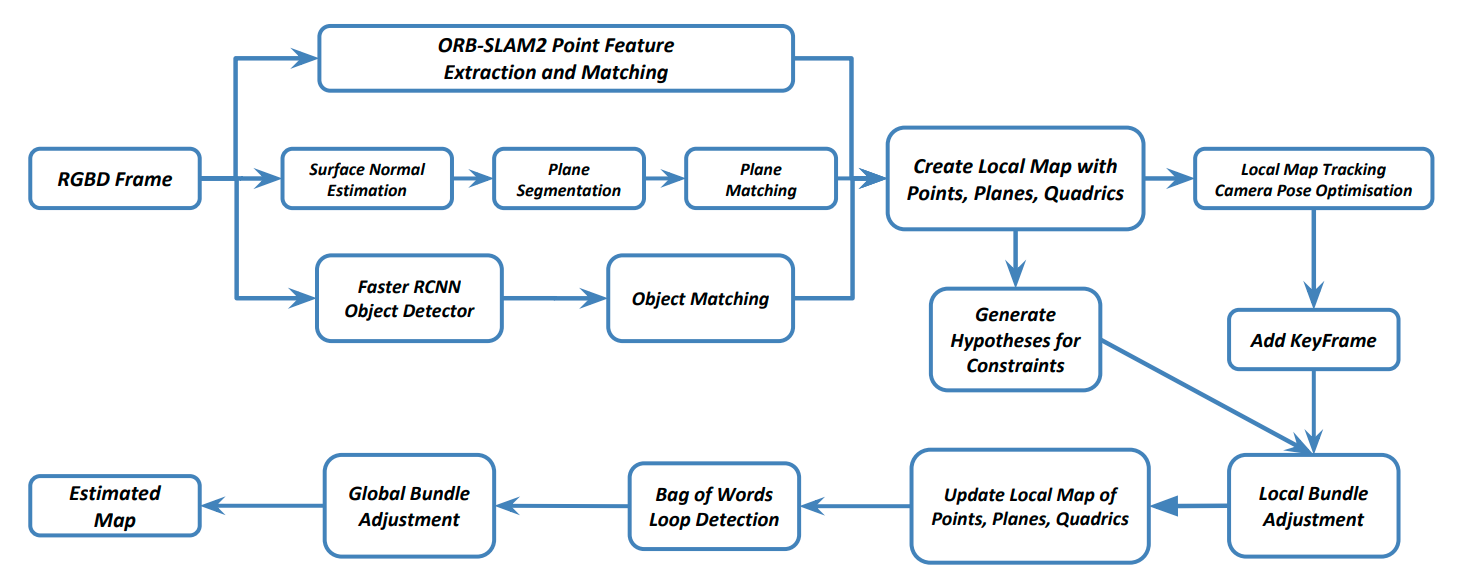
\includegraphics[scale=0.3] {Images/structure_aware_slam.png}
\caption{\centering Structure Aware SLAM pipeline \cite{StructureAS}}
\label{fig:structure_aware_slam.png}
\end{figure}
    
\end{document}
